In \autoref{tab:freq} befinden sich die Wellenlängen, die Frequenz und die zugehörige Grenzspannung. 
\begin{table}
    \centering 
    \caption{Wellenlänge, Frequenz und zugehörige Grenzspannung.}
\begin{tabular}{c c c}
    \toprule
    $\lambda$ in nm &$\nu$ in $10^14\cdot$\,Hz & $U_{\symup{g}}$ in V  \\
    \midrule
    700 & 4.28271 & 0.8158\\ 
546 & 5.49066 & 0.693\\
435 & 6.89172 & 1.2215\\
    \bottomrule
\end{tabular}
\label{tab:freq}
\end{table}

Die Frequenz wurde dabei mit
\begin{equation*}
    \nu = \frac{\symup{c}}{\lambda}
\end{equation*}
berechnet. Die Wellenlängen wurden vorwiegend der Versuchsanleitung \cite{ap500} entnommen. Für die Wellenlänge von rotem Licht wurde 
$700\,\unit{\nm}$ \cite{rot} gewählt.
In \autoref{fig:freq} wurde nun der jeweilige Betrag Grenzspannung gegen die Frequenz aufgetragen und eine Ausgleichsrechnung mittels einer Geraden
durchgeführt. Dabei wurde die Grenzspannung der grünen Spektrallinie für die Ausgleichsrechnung nicht beachtet, da sie sehr stark von dem Verlauf der 
anderen Messungen sowie der theoretischen Erwartung, dass die Grenzspannung linear mit der Frequenz steigt, abweicht.
\begin{figure}
    \centering
    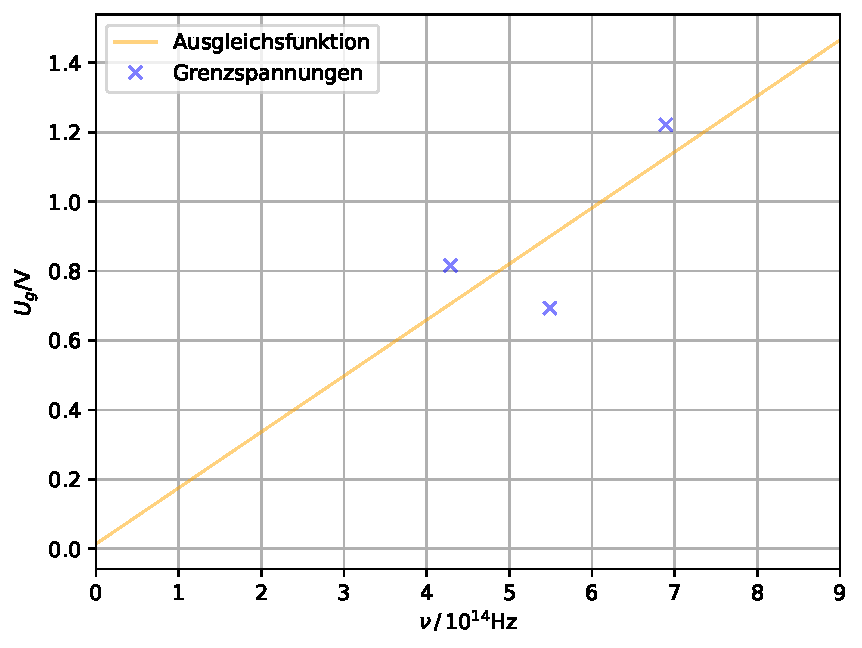
\includegraphics[height = 8cm]{build/frequenz.pdf}
    \caption{Verlauf der Grenzspannungen in Abhängigkeit von der Frequenz.}
    \label{fig:freq}
\end{figure}
Dabei ergeben sich für die Steigung, welcher hier das Verhältnis $\frac{h}{\symup{e_0}}$ darstellt 
\begin{equation*}
    a = \frac{h}{\symup{e_0}} = 1.555 \cdot 10^{-15} \,\unit{\eV}
\end{equation*}
und den y-Achsenabschnitt
\begin{equation*}
    b = A_{\symup{k}} = 1.498 \,\unit{\eV} \; ,
\end{equation*}
welcher hier der Austrittsarbeit $A_{\symup{k}}$ entspricht.

Da bei der Ausgleichsrechnung nur zwei Werte betrachtet wurden, kann keine Fehlerabweichung angegeben werden.



In \autoref{fig:gelb} wird der Verlauf des Photostroms bei einer Wellenlänge von $\lambda = 578 \,\unit{\nm}$ dargestellt. Dabei wurde ein größeres 
Intervall der anliegenden Spannung betrachtet. Die dazu gehörenden Messwerte finden sich in \autoref{tab:gelb}.

\begin{table}
    \centering 
    \caption{Messwerte der gelben Spektrallinie.}
\begin{tabular}{c c}
    \toprule
    $U$ in V&$I$ in pA \\
    \midrule
    0&60 \\
    1&180 \\
    2&280 \\
  2.5&320 \\
    3&380 \\
  3.5&400 \\
    4&440 \\
  4.5&440 \\
    5&460 \\
    6&500 \\
    7&520 \\
    8&540 \\
    9&560 \\
   10&580 \\
   11&580 \\
   12&640 \\
   13&640 \\
   14&660 \\
   15&660 \\
   16&680 \\
   17&700 \\
   18&700 \\
   19&720 \\
    0&180 \\
    -1&20 \\
    -3&20 \\
    -4&15 \\
    -5&15 \\
    -6&15 \\
    -7&15 \\
    -8&15 \\
    -9&18 \\
   -10&18 \\
   -11&18 \\
   -12&20 \\
   -13&20 \\
   -14&20 \\
   -15&20 \\
   -16&20 \\
   -17&20 \\
   -18&20 \\
   -19&20 \\
    \bottomrule
\end{tabular}
\label{tab:gelb}
\end{table}

    
\begin{figure}
    \centering
    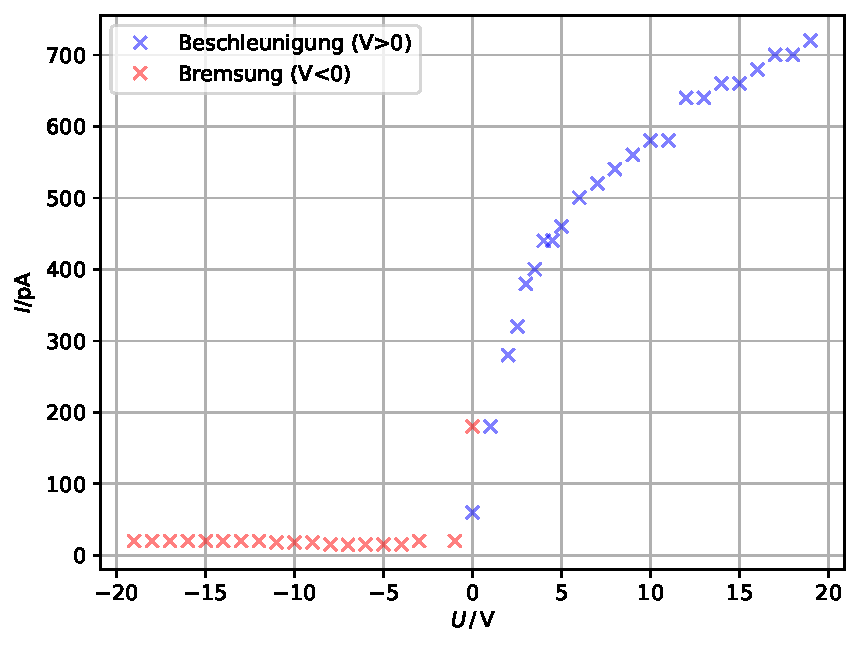
\includegraphics[height = 8cm]{build/plotgelb.pdf}
    \caption{Verlauf des Photostroms der gelben Spektrallinie bei $\lambda = 578 \,\unit{\nm}$.}
    \label{fig:gelb}
\end{figure}
Bei hohen beschleunigenden Spannung erreicht der Photostrom asymptotisch einen Sättigungswert. Dies liegt daran, dass ab einer bestimmten
Beschleunigungsspannung alle Elektronen die Anode erreichen. Nach der Korpuskeltheorie ist die Anzahl der Elektronen proportional zur Intensität 
des Lichts, sodass bei konstanter Lichteinstrahlung der obigen Wellenlänge der Strom nicht über einen bestimmten Wert hinauswachsen kann. In 
\autoref{fig:gelb} erkennt man bei großen Beschleunigungsspannungen langsam eine Abflachung des Strom; der Sättigungswert ist jedoch noch nicht ganz erkennbar.
Die Annäherung an dem Sättigungswert erfolgt asymptotisch und der Sättigungswert kann in der Praxis nicht vollständig erreicht werden. Dies liegt daran ,dass 
nicht alle Elektronen durch etwaige Ablenkungen und Widerstände die Anode erreichen können. Bei hohen Beschleunigungen haben diese aber einen immer geringeren 
Einfluss. Um den Sättigungswert zu erreichen müssen also alle Widerstände und Ablenkungen eliminiert werden. Das ist nur im Vakuum und bei einer ausreichenden 
Isolierung und Abschirmung von anderen Lichtquellen der  gesamten Messapparatur möglich.

Der Photostrom fällt bi $U_{\symup{g}}$ nicht direkt auf Null ab, da die Elektronen schon vor der Emission aus dem Material eine gewisse Energie 
haben, welche der Fermi-Dirac-Statistik folgt. Dadurch werden größere Bremsspannungen benötigt, um alle Elektronen soweit auszubremsen, dass sie die 
Anode nicht erreichen. In \autoref{fig:gelb} wird die Null gar nicht erreicht, da die Bremsspannungen scheinbar noch nicht groß genug sind. Dennoch erkennt 
man direkt unter einer Spannung von $0\,\unit{\volt}$ einen etwas höheren Photostrom als bei größeren Bremsspannungen, was darauf hindeutet, dass 
der Photostrom noch weiter abfallen wird, wenn die Bremsspannung weiter erhöht werden würde.

Grundsätzlich kann ein kleiner entgegengerichteter Strom bei hohen Bremsspannungen gemessen werden. Bei dem Versuchsteil zur gelben Spektrallinie wurde dies jedoch nicht beobachtet 
Bei der violetten Spektrallinie in \autoref{tab:lila} jedoch schon. Dieser ist damit zu erklären, dass das Kathodenmaterial bei $T=20°\,\unit{\celsius}$ 
verdampft, wodurch Elektronen freigesetzt werden und sich an der Anode anlagern. Das führt dazu, dass die Elektronen wegen der hohen Bremsspannung von der 
Anode wegbeschleunigt werden und es wird ein negativer Strom gemessen. Dadurch dass hierbei wesentlich weniger Elektronen zu beobachten sind, kann hier 
der Sättigungswert erreicht werden. 

Da der negative Strom bereits bei energiearmen Licht beobachtet werden kann, muss die Austrittsarbeit mindestens so klein wie die der Kathode sein.